\documentclass[a4paper,12pt,twocolumn]{article}

\usepackage[landscape,top=1cm,bottom=1.4cm,left=1cm,right=1cm,columnsep=1cm]{geometry}
\usepackage[fleqn]{amsmath}
\usepackage{amssymb}
\setlength{\mathindent}{1.5em}
\usepackage{fontspec}
\usepackage{enumitem}
\usepackage{framed}
\usepackage{needspace}
\usepackage[hidelinks]{hyperref}
\usepackage{tikz}
\usepackage{pgfplots}
\usepgfplotslibrary{groupplots}

\setmainfont{Times New Roman}
\setsansfont{Arial}

\pgfplotsset{compat=1.18}

\pagestyle{plain}
\setlength{\columnseprule}{0.2pt}
\newcommand{\examdate}{2026/04/22}
\newlength{\problemnumberwidth}
\settowidth{\problemnumberwidth}{\textbf{78.}\ }
\newenvironment{solutionbox}{\begin{framed}}{\end{framed}}

\newcommand{\sectiontitle}[2]{%
  \hypertarget{#1}{}%
  \par\vspace{0.8em}%
  \noindent{\Large\bfseries #2}\par
  \vspace{0.3em}%
  \hrule
  \vspace{0.8em}%
}

\newcommand{\tocproblem}[2]{%
  \hyperref[#1]{#2} & \hyperref[#1]{\pageref*{#1}} \\
}

\newcommand{\worksheettoc}{%
  \noindent{\Large\bfseries Contents}\par
  \vspace{0.3em}%
  \hrule
  \vspace{0.9em}%
  \begin{tabular}{@{}p{0.72\columnwidth}r@{}}
    \textbf{Problem} & \textbf{Page} \\
    \tocproblem{prob:14-1-32}{14-1 \quad 32}
    \tocproblem{prob:14-1-48}{14-1 \quad 48}
    \tocproblem{prob:14-1-49}{14-1 \quad 49}
    \tocproblem{prob:14-1-52}{14-1 \quad 52}
    \tocproblem{prob:14-1-56}{14-1 \quad 56}
    \tocproblem{prob:14-1-78}{14-1 \quad 78}
    \tocproblem{prob:14-2-23}{14-2 \quad 23}
    \tocproblem{prob:14-2-24}{14-2 \quad 24}
    \tocproblem{prob:14-2-30}{14-2 \quad 30}
    \tocproblem{prob:14-2-42}{14-2 \quad 42}
    \tocproblem{prob:14-2-48}{14-2 \quad 48}
    \tocproblem{prob:14-2-49}{14-2 \quad 49}
  \end{tabular}\par
}

\newcommand{\problem}[3]{%
  \Needspace{10\baselineskip}%
  \phantomsection\label{#1}%
  \par\vspace{0.8em}%
  \noindent
  \hangindent=\problemnumberwidth
  \hangafter=1
  \makebox[\problemnumberwidth][l]{\textbf{#2.}}#3\par
}

\newlist{subparts}{enumerate}{1}
\setlist[subparts]{%
  label = (\alph*),
  labelindent=\problemnumberwidth,
  leftmargin=*,
  labelsep=0.5em,
  align=left,
  itemsep=0.2em,
  topsep=0.3em,
  parsep=0pt,
  partopsep=0pt
}

\newlist{steps}{enumerate}{1}
\setlist[steps]{%
  label=\textbf{Step \arabic*.},
  leftmargin=*,
  itemsep=0.35em,
  topsep=0.35em,
  align=left
}

\pgfplotsset{
  worksheet surface/.style={
    width=3.45cm,
    height=2.85cm,
    xmin=-2.25,
    xmax=2.25,
    ymin=-2.25,
    ymax=2.25,
    domain=-2.25:2.25,
    y domain=-2.25:2.25,
    samples=9,
    samples y=9,
    ticks=none,
    axis lines=none,
    title style={font=\bfseries\large},
    scale only axis,
    clip=false,
    z buffer=sort,
    unbounded coords=jump
  },
  worksheet floor/.style={
    mesh,
    samples=7,
    samples y=7,
    draw=black!22,
    opacity=0.8
  },
  worksheet colored surface/.style={
    surf,
    samples=11,
    samples y=11,
    point meta/expr={0.55*x + 0.35*y + 1.10*z},
    shader=interp,
    fill opacity=0.52,
    draw=none,
    colormap={worksheetpos}{
      color (0cm) = (cyan!35!white);
      color (0.35cm) = (blue!70!cyan);
      color (0.7cm) = (magenta!75!blue);
      color (1cm) = (yellow!70!magenta)
    }
  },
  worksheet axis/.style={
    ->,
    black,
    line width=0.35pt
  }
}

\newcommand{\surfaceaxes}[2]{%
  \addplot3[worksheet floor] {#1};
  \addplot3[worksheet axis] coordinates {(-2.2,0,#1) (2.45,0,#1)}
    node[pos=1, anchor=west, font=\tiny] {$x$};
  \addplot3[worksheet axis] coordinates {(0,-2.2,#1) (0,2.45,#1)}
    node[pos=1, anchor=south west, font=\tiny] {$y$};
  \addplot3[worksheet axis] coordinates {(0,0,#1) (0,0,#2)}
    node[pos=1, anchor=south, font=\tiny] {$z$};
}

\newcommand{\matchgraphsfigure}{%
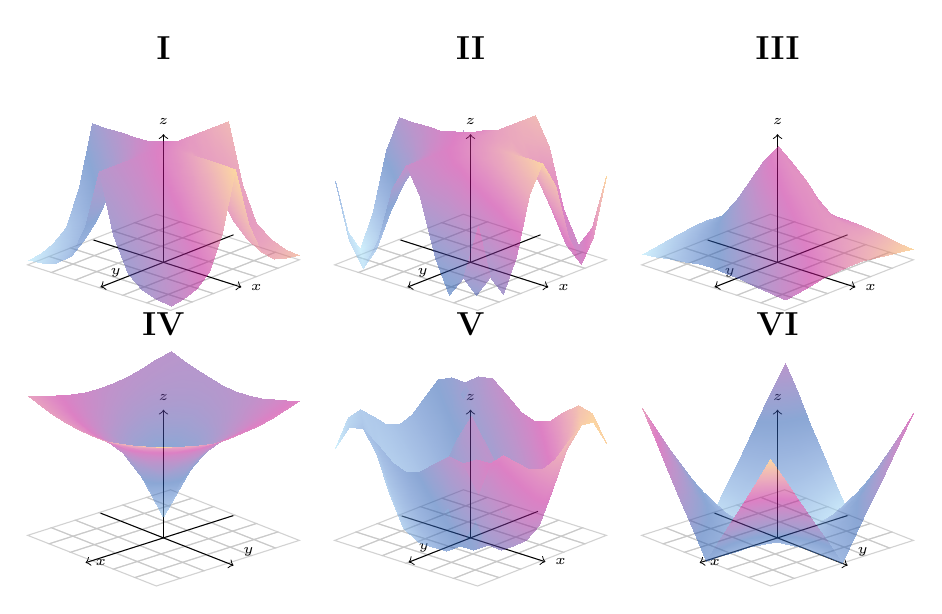
\begin{tikzpicture}
  \begin{groupplot}[
    group style={group size=3 by 2, horizontal sep=0.45cm, vertical sep=0.65cm}
  ]

    \nextgroupplot[
      worksheet surface,
      title={I},
      view={42}{28},
      zmin=0,
      zmax=1.1
    ]
    \surfaceaxes{0}{1.1}
    \addplot3[worksheet colored surface] {1/(1 + x^2*y^2)};

    \nextgroupplot[
      worksheet surface,
      title={II},
      view={42}{28},
      zmin=-1.1,
      zmax=1.1
    ]
    \surfaceaxes{-1.1}{1.1}
    \addplot3[worksheet colored surface] {cos(deg(x*y))};

    \nextgroupplot[
      worksheet surface,
      title={III},
      view={42}{28},
      zmin=0,
      zmax=1.1
    ]
    \surfaceaxes{0}{1.1}
    \addplot3[worksheet colored surface] {1/(1 + x^2 + y^2)};

    \nextgroupplot[
      worksheet surface,
      title={IV},
      view={138}{28},
      zmin=-4.2,
      zmax=1.8
    ]
    \surfaceaxes{-4.2}{1.8}
    \addplot3[worksheet colored surface] {ln(max(x^2 + y^2, 0.04))};

    \nextgroupplot[
      worksheet surface,
      title={V},
      view={42}{28},
      xmin=-5.2,
      xmax=5.2,
      ymin=-5.2,
      ymax=5.2,
      domain=-5.2:5.2,
      y domain=-5.2:5.2,
      zmin=-1.1,
      zmax=1.1
    ]
    \addplot3[worksheet floor, domain=-5.2:5.2, y domain=-5.2:5.2] {-1.1};
    \addplot3[worksheet axis] coordinates {(-5.0,0,-1.1) (5.45,0,-1.1)}
      node[pos=1, anchor=west, font=\tiny] {$x$};
    \addplot3[worksheet axis] coordinates {(0,-5.0,-1.1) (0,5.45,-1.1)}
      node[pos=1, anchor=south west, font=\tiny] {$y$};
    \addplot3[worksheet axis] coordinates {(0,0,-1.1) (0,0,1.1)}
      node[pos=1, anchor=south, font=\tiny] {$z$};
    \addplot3[worksheet colored surface, samples=11, samples y=11]
      {cos(deg(sqrt(x^2 + y^2)))};

    \nextgroupplot[
      worksheet surface,
      title={VI},
      view={138}{28},
      zmin=0,
      zmax=5.1
    ]
    \surfaceaxes{0}{5.1}
    \addplot3[worksheet colored surface] {abs(x*y)};
  \end{groupplot}
\end{tikzpicture}%
}

\begin{document}

\twocolumn[
{\centering
\Large\bfseries Calculus Problems Solutions\par
\vspace{0.5em}
\noindent\hfill\normalsize\normalfont \examdate\par
\vspace{0.8em}
}
]

\worksheettoc
\vfill\null
\newpage

\sectiontitle{sec:14-1}{14-1}

\problem{prob:14-1-32}{32}{Match the function with its graph (labeled I--VI). Give reasons for your choices.
\[
\begin{alignedat}{2}
(a)\quad & f(x,y)=\frac{1}{1+x^2+y^2} \qquad &
(b)\quad & f(x,y)=\frac{1}{1+x^2y^2} \\
(c)\quad & f(x,y)=\ln(x^2+y^2) \qquad &
(d)\quad & f(x,y)=\cos \sqrt{x^2+y^2} \\
(e)\quad & f(x,y)=|xy| \qquad &
(f)\quad & f(x,y)=\cos(xy)
\end{alignedat}
\]}

\begin{center}
\matchgraphsfigure
\end{center}

\begin{solutionbox}
\textbf{Method 1: Match by symmetry, sign, and special cross-sections}

\begin{steps}
\item First separate the radially symmetric functions from the nonradial ones. Functions
\[
\frac{1}{1+x^2+y^2},\qquad \ln(x^2+y^2),\qquad \cos\sqrt{x^2+y^2}
\]
depend only on \(x^2+y^2\), so their graphs must look the same in every horizontal direction. That is the fastest first cut because only some of the six graphs have circular symmetry.

\item For
\[
f(x,y)=\frac{1}{1+x^2+y^2},
\]
the value is positive everywhere, equals \(1\) at the origin, and decreases to \(0\) as \(x^2+y^2\to\infty\). So it must be the single smooth hill with highest point at the center. That matches graph \(\mathrm{III}\).

\item For
\[
f(x,y)=\ln(x^2+y^2),
\]
the graph is radially symmetric again, but now \(f(x,y)\to-\infty\) as \((x,y)\to(0,0)\), and \(f\) increases as we move outward. So the graph must have a deep pit at the origin rather than a hill. That matches graph \(\mathrm{IV}\).

\item For
\[
f(x,y)=\cos\sqrt{x^2+y^2},
\]
the graph is radially symmetric and oscillates as the distance from the origin increases. Therefore the surface should show concentric ripples with alternating peaks and valleys. That matches graph \(\mathrm{V}\).

\item Now look at the nonradial functions. For
\[
f(x,y)=\frac{1}{1+x^2y^2},
\]
we still have \(0<f\le 1\), but along either axis \(x=0\) or \(y=0\) we get \(f=1\). So instead of one isolated central peak, the graph has two perpendicular ridges of height \(1\). That is graph \(\mathrm{I}\).

\item For
\[
f(x,y)=|xy|,
\]
the function is always nonnegative and vanishes on both coordinate axes. Away from the axes, it rises in all four quadrants. So the graph looks like four upward-curving sheets meeting along the axes, which is graph \(\mathrm{VI}\).

\item Finally,
\[
f(x,y)=\cos(xy)
\]
has the same special feature \(f=1\) on both axes, but unlike part (b) it oscillates between positive and negative values as \(|xy|\) grows. So the surface has ridges on the axes together with alternating waves farther out. That matches graph \(\mathrm{II}\).
\end{steps}
\end{solutionbox}

\begin{solutionbox}
\textbf{Method 2: Match by level curves}

\begin{steps}
\item The level curves of
\[
\frac{1}{1+x^2+y^2}=k
\]
are circles
\[
x^2+y^2=\frac{1}{k}-1,
\qquad 0<k\le 1.
\]
Circular level curves with larger values near the center mean a dome-shaped radial hill, so this must be graph \(\mathrm{III}\).

\item The level curves of
\[
\ln(x^2+y^2)=k
\]
are also circles:
\[
x^2+y^2=e^k.
\]
Since \(k\to-\infty\) corresponds to circles shrinking toward the origin, the origin is the place where the surface plunges downward. Hence this is graph \(\mathrm{IV}\).

\item The level curves of
\[
\cos\sqrt{x^2+y^2}=k
\]
are again circles, but now many different radii can give the same value because cosine oscillates. So the graph must have concentric wave rings. That identifies graph \(\mathrm{V}\).

\item For
\[
\frac{1}{1+x^2y^2}=k,
\]
we get
\[
x^2y^2=\frac{1}{k}-1
\qquad\Longrightarrow\qquad
|xy|=\sqrt{\frac{1}{k}-1}.
\]
These are hyperbolas, while the axes themselves give the maximum value \(1\). A surface with hyperbolic level sets and high ridges on the axes is graph \(\mathrm{I}\).

\item For
\[
|xy|=k,
\]
the level curves are again hyperbolas, but now the function is \(0\) on the axes and grows without bound away from them. So the graph has valleys along the axes and rises in the quadrants. That is graph \(\mathrm{VI}\).

\item For
\[
\cos(xy)=k,
\]
the level curves satisfy
\[
xy=\pm\arccos(k)+2\pi n
\]
for integers \(n\). These are alternating families of hyperbolas, which explains the oscillating wave pattern based on \(xy\). Therefore the remaining graph is \(\mathrm{II}\).
\end{steps}
\end{solutionbox}

\begin{solutionbox}
\textbf{Hand-in Version}

The correct matches are
\[
\boxed{(a)\to \mathrm{III},\quad (b)\to \mathrm{I},\quad (c)\to \mathrm{IV}}
\]
\[
\boxed{(d)\to \mathrm{V},\quad (e)\to \mathrm{VI},\quad (f)\to \mathrm{II}}
\]

Reasons:
\[
\frac{1}{1+x^2+y^2}
\]
is the only positive radially symmetric hill, so it is \(\mathrm{III}\). The function
\[
\ln(x^2+y^2)
\]
is radially symmetric with a vertical drop to \(-\infty\) at the origin, so it is \(\mathrm{IV}\). The function
\[
\cos\sqrt{x^2+y^2}
\]
is radially symmetric and oscillatory, so it is \(\mathrm{V}\).

For the nonradial graphs,
\[
\frac{1}{1+x^2y^2}=1
\]
on both axes, so it has two ridges and matches \(\mathrm{I}\). The function
\[
|xy|
\]
is \(0\) on the axes and positive in the four quadrants, so it is \(\mathrm{VI}\). Finally,
\[
\cos(xy)
\]
also equals \(1\) on the axes but oscillates as \(|xy|\) grows, so it is \(\mathrm{II}\).
\end{solutionbox}

\problem{prob:14-1-48}{48}{Draw a contour map of the function showing several level curves.
\[
f(x,y)=\ln(x^2+4y^2)
\]}

\begin{solutionbox}
\textbf{Method 1: Set the function equal to a constant}

\begin{steps}
\item A contour map is made from level curves, so we set
\[
\ln(x^2+4y^2)=k,
\]
where \(k\) is a constant. This is the right starting point because a contour map is literally the collection of these equations for different values of \(k\).

\item Exponentiating gives
\[
x^2+4y^2=e^k.
\]
Now the geometry becomes transparent: each level curve is an ellipse centered at the origin.

\item Rewrite it in standard form:
\[
\frac{x^2}{e^k}+\frac{y^2}{e^k/4}=1.
\]
So the semiaxis lengths are
\[
a=\sqrt{e^k}=e^{k/2},
\qquad
b=\frac12 e^{k/2}.
\]
This explains why every contour is stretched farther in the \(x\)-direction than in the \(y\)-direction.

\item As \(k\) increases, \(e^k\) increases, so the ellipses get larger. As \(k\to-\infty\), the ellipses shrink toward the origin. That tells us how to label the nested contours: larger \(k\) means farther from the origin.
\end{steps}
\end{solutionbox}

\begin{solutionbox}
\textbf{Method 2: Convert the problem into circles}

\begin{steps}
\item Introduce a new variable
\[
v=2y.
\]
Then the function becomes
\[
f(x,y)=\ln(x^2+v^2).
\]
This substitution is appropriate because it removes the coefficient \(4\) and turns the inside into the ordinary radial form \(x^2+v^2\).

\item In the \((x,v)\)-plane, the level curves satisfy
\[
x^2+v^2=e^k,
\]
which are circles centered at the origin.

\item When we translate back to \(v=2y\), each circle becomes an ellipse in the original \((x,y)\)-plane. Circles stay centered at the origin, but the \(v\)-direction is compressed by a factor of \(2\), so the \(y\)-semiaxis is only half as long as the \(x\)-semiaxis.

\item Therefore the contour map consists of nested ellipses centered at the origin, elongated horizontally.
\end{steps}
\end{solutionbox}

\begin{solutionbox}
\textbf{Hand-in Version}

Let
\[
\ln(x^2+4y^2)=k.
\]
Then
\[
x^2+4y^2=e^k,
\]
so each level curve is an ellipse centered at the origin. In standard form,
\[
\frac{x^2}{e^k}+\frac{y^2}{e^k/4}=1,
\]
so the semiaxes are \(e^{k/2}\) in the \(x\)-direction and \(\tfrac12 e^{k/2}\) in the \(y\)-direction. Thus the contour map is a family of horizontally stretched concentric ellipses, with larger values of \(k\) farther from the origin.

\begin{center}
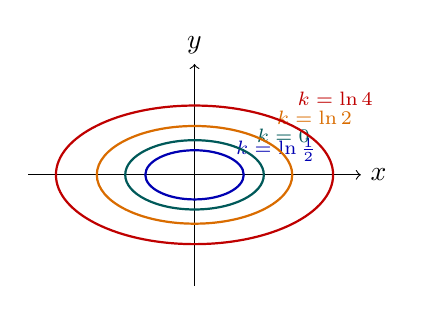
\begin{tikzpicture}[scale=0.88]
  \draw[->] (-2.4,0) -- (2.4,0) node[right] {\(x\)};
  \draw[->] (0,-1.6) -- (0,1.6) node[above] {\(y\)};

  \draw[thick,blue!70!black] (0,0) ellipse [x radius=0.71, y radius=0.355];
  \node[blue!70!black] at (1.18,0.36) {\scriptsize \(k=\ln \frac12\)};

  \draw[thick,teal!70!black] (0,0) ellipse [x radius=1.00, y radius=0.50];
  \node[teal!70!black] at (1.28,0.56) {\scriptsize \(k=0\)};

  \draw[thick,orange!85!black] (0,0) ellipse [x radius=1.41, y radius=0.705];
  \node[orange!85!black] at (1.73,0.82) {\scriptsize \(k=\ln 2\)};

  \draw[thick,red!75!black] (0,0) ellipse [x radius=2.00, y radius=1.00];
  \node[red!75!black] at (2.03,1.10) {\scriptsize \(k=\ln 4\)};
\end{tikzpicture}
\end{center}
\end{solutionbox}

\problem{prob:14-1-49}{49}{Draw a contour map of the function showing several level curves.
\[
f(x,y)=ye^x
\]}

\begin{solutionbox}
\textbf{Method 1: Solve the level equation for \(y\)}

\begin{steps}
\item Set
\[
ye^x=k.
\]
This is the natural first step because a contour map is built from all points that give the same function value.

\item Solve for \(y\):
\[
y=ke^{-x}.
\]
So every level curve is an exponential graph.

\item The sign of \(y\) must match the sign of \(k\), because \(e^x>0\) for every real \(x\). Therefore positive level curves lie above the \(x\)-axis, negative level curves lie below it, and \(k=0\) gives the \(x\)-axis itself.

\item As \(x\to\infty\), \(e^{-x}\to 0\), so every nonzero level curve approaches the \(x\)-axis. As \(x\to-\infty\), \(|ke^{-x}|\to\infty\), so the curves rise or fall sharply on the left. This explains the overall contour-map shape.
\end{steps}
\end{solutionbox}

\begin{solutionbox}
\textbf{Method 2: Compare all contours to one basic curve}

\begin{steps}
\item The level equation is again
\[
y=ke^{-x}.
\]
Write it as
\[
y=k\bigl(e^{-x}\bigr).
\]
This viewpoint is useful because it shows all nonzero contours are vertical scalings of the single base curve \(y=e^{-x}\).

\item That means every positive contour has the same shape as every other positive contour, just multiplied by a different constant \(k\). Likewise, every negative contour is the reflection of a positive one across the \(x\)-axis.

\item Differentiate implicitly along a contour:
\[
\frac{dy}{dx}=-ke^{-x}=-y.
\]
So when \(y>0\), the contour slopes downward; when \(y<0\), it slopes upward. This confirms the geometry of the sketch rather than just the algebra.

\item Therefore the contour map consists of a stack of decreasing exponentials above the axis, their reflections below the axis, and the \(x\)-axis for the zero level.
\end{steps}
\end{solutionbox}

\begin{solutionbox}
\textbf{Hand-in Version}

The level curves satisfy
\[
ye^x=k
\qquad\Longrightarrow\qquad
y=ke^{-x}.
\]
So each contour is an exponential curve. If \(k>0\), the contour lies above the \(x\)-axis; if \(k<0\), it lies below the \(x\)-axis; and if \(k=0\), the contour is the \(x\)-axis itself. As \(x\to\infty\), every nonzero contour approaches \(y=0\).

\begin{center}
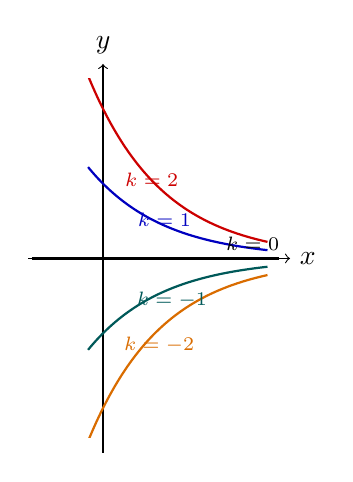
\begin{tikzpicture}[scale=0.95]
  \draw[->] (-1.0,0) -- (2.5,0) node[right] {\(x\)};
  \draw[->] (0,-2.6) -- (0,2.6) node[above] {\(y\)};

  \begin{scope}
    \clip (-1.0,-2.4) rectangle (2.4,2.4);
    \draw[thick,red!80!black,samples=120,domain=-0.2:2.2,smooth]
      plot (\x,{2*exp(-\x)});
    \draw[thick,blue!75!black,samples=120,domain=-0.2:2.2,smooth]
      plot (\x,{exp(-\x)});
    \draw[thick,black] (-0.95,0) -- (2.35,0);
    \draw[thick,teal!70!black,samples=120,domain=-0.2:2.2,smooth]
      plot (\x,{-exp(-\x)});
    \draw[thick,orange!85!black,samples=120,domain=-0.2:2.2,smooth]
      plot (\x,{-2*exp(-\x)});
  \end{scope}

  \node[red!80!black] at (0.65,1.05) {\scriptsize \(k=2\)};
  \node[blue!75!black] at (0.82,0.52) {\scriptsize \(k=1\)};
  \node[black] at (2.00,0.20) {\scriptsize \(k=0\)};
  \node[teal!70!black] at (0.92,-0.55) {\scriptsize \(k=-1\)};
  \node[orange!85!black] at (0.75,-1.15) {\scriptsize \(k=-2\)};
\end{tikzpicture}
\end{center}
\end{solutionbox}

\problem{prob:14-1-52}{52}{Draw a contour map of the function showing several level curves.
\[
f(x,y)=\frac{y}{x^2+y^2}
\]}

\begin{solutionbox}
\textbf{Method 1: Complete the square in the level equation}

\begin{steps}
\item Set
\[
\frac{y}{x^2+y^2}=k.
\]
This is the correct first step because a contour map comes from solving the equation \(f(x,y)=k\).

\item If \(k\ne 0\), multiply through:
\[
y=k(x^2+y^2).
\]
Move everything to one side:
\[
x^2+y^2-\frac{1}{k}y=0.
\]

\item Complete the square in \(y\):
\[
x^2+\left(y-\frac{1}{2k}\right)^2=\frac{1}{4k^2}.
\]
So every nonzero level curve is a circle centered at
\[
\left(0,\frac{1}{2k}\right)
\]
with radius
\[
\frac{1}{2|k|}.
\]
This is an important structural fact: all contours are circles tangent to the origin.

\item When \(k=0\), the equation becomes \(y=0\). Since the original function is undefined at \((0,0)\), the zero contour is the \(x\)-axis with the origin removed. So the contour map is a family of tangent circles above and below the axis together with the punctured \(x\)-axis.
\end{steps}
\end{solutionbox}

\begin{solutionbox}
\textbf{Method 2: Use polar coordinates}

\begin{steps}
\item Write
\[
x=r\cos\theta,\qquad y=r\sin\theta.
\]
Then
\[
f(x,y)=\frac{r\sin\theta}{r^2}=\frac{\sin\theta}{r},
\qquad r>0.
\]
Polar coordinates are appropriate here because the denominator \(x^2+y^2\) becomes the simple quantity \(r^2\).

\item Setting \(f=k\) gives
\[
\frac{\sin\theta}{r}=k
\qquad\Longrightarrow\qquad
r=\frac{1}{k}\sin\theta
\qquad (k\ne 0).
\]

\item The polar equation
\[
r=2a\sin\theta
\]
represents a circle of radius \(a\) centered at \((0,a)\). Here
\[
2a=\frac{1}{k}
\qquad\Longrightarrow\qquad
a=\frac{1}{2k}.
\]
So we recover exactly the same circles as in Method 1.

\item The sign of \(k\) decides whether the circle lies above or below the \(x\)-axis, because the center is at \(y=\frac{1}{2k}\). This gives a quick way to sketch the whole contour family.
\end{steps}
\end{solutionbox}

\begin{solutionbox}
\textbf{Hand-in Version}

For the level curve \(f(x,y)=k\),
\[
\frac{y}{x^2+y^2}=k.
\]
If \(k\ne 0\), then
\[
y=k(x^2+y^2)
\]
and completing the square gives
\[
\boxed{x^2+\left(y-\frac{1}{2k}\right)^2=\frac{1}{4k^2}.}
\]
So every nonzero level curve is a circle tangent to the origin, centered on the \(y\)-axis. If \(k>0\), the circle is above the \(x\)-axis; if \(k<0\), it is below. For \(k=0\), the contour is \(y=0\) with the origin excluded.

\begin{center}
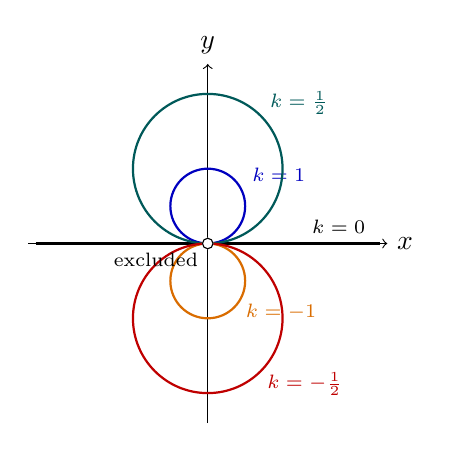
\begin{tikzpicture}[scale=0.95]
  \draw[->] (-2.4,0) -- (2.4,0) node[right] {\(x\)};
  \draw[->] (0,-2.4) -- (0,2.4) node[above] {\(y\)};

  \draw[thick,black] (-2.3,0) -- (2.3,0);
  \node[black] at (1.75,0.22) {\scriptsize \(k=0\)};

  \draw[thick,blue!75!black] (0,0.5) circle[radius=0.5];
  \node[blue!75!black] at (0.95,0.92) {\scriptsize \(k=1\)};

  \draw[thick,teal!70!black] (0,1.0) circle[radius=1.0];
  \node[teal!70!black] at (1.22,1.88) {\scriptsize \(k=\frac12\)};

  \draw[thick,orange!85!black] (0,-0.5) circle[radius=0.5];
  \node[orange!85!black] at (0.98,-0.92) {\scriptsize \(k=-1\)};

  \draw[thick,red!75!black] (0,-1.0) circle[radius=1.0];
  \node[red!75!black] at (1.30,-1.88) {\scriptsize \(k=-\frac12\)};

  \filldraw[white] (0,0) circle (2pt);
  \draw (0,0) circle (2pt);
  \node[below left] at (0,0) {\scriptsize excluded};
\end{tikzpicture}
\end{center}
\end{solutionbox}

\problem{prob:14-1-56}{56}{If \(V(x,y)\) is the electric potential at a point \((x,y)\) in the \(xy\)-plane, then the level curves of \(V\) are called equipotential curves because at all points on such a curve the electric potential is the same. Sketch some equipotential curves if
\[
V(x,y)=\frac{c}{\sqrt{r^2-x^2-y^2}},
\]
where \(c\) is a positive constant.}

\begin{solutionbox}
\textbf{Method 1: Solve the level equation directly}

\begin{steps}
\item To avoid confusing the constant \(r\) in the formula with the polar radius, let us temporarily rename that constant \(R>0\). Then
\[
V(x,y)=\frac{c}{\sqrt{R^2-x^2-y^2}}.
\]
This is appropriate because the geometry is easier to describe when the symbols do not collide.

\item Set \(V(x,y)=K\), where \(K\) is a constant potential. Then
\[
\frac{c}{\sqrt{R^2-x^2-y^2}}=K.
\]
Since the left-hand side is positive, only positive \(K\) can occur.

\item Solve for the curve:
\[
\sqrt{R^2-x^2-y^2}=\frac{c}{K}
\]
and then
\[
x^2+y^2=R^2-\frac{c^2}{K^2}.
\]
So every equipotential curve is a circle centered at the origin.

\item The radius is
\[
\rho=\sqrt{R^2-\frac{c^2}{K^2}}.
\]
For this radius to be real, we must have
\[
R^2-\frac{c^2}{K^2}\ge 0
\qquad\Longleftrightarrow\qquad
K\ge \frac{c}{R}.
\]
Thus not every positive \(K\) gives a level curve. If \(K=\frac{c}{R}\), then \(\rho=0\), so the level set is only the origin. If \(K>\frac{c}{R}\), we get a genuine circle. If \(0<K<\frac{c}{R}\), there is no real level curve.

\item Since larger \(K\) makes \(\frac{c^2}{K^2}\) smaller, the radius increases with \(K\). This matches the original formula: the potential gets larger as we move closer to the boundary \(x^2+y^2=R^2\).

\item The domain is
\[
x^2+y^2<R^2.
\]
At the origin the potential is smallest:
\[
V(0,0)=\frac{c}{R},
\]
and as \(\rho\to R^{-}\), the potential tends to \(+\infty\). So the equipotential circles are concentric circles inside the disk \(x^2+y^2<R^2\), becoming denser near the outer boundary.
\end{steps}
\end{solutionbox}

\begin{solutionbox}
\textbf{Method 2: Use radial symmetry first}

\begin{steps}
\item Notice that \(V\) depends on \(x\) and \(y\) only through
\[
x^2+y^2.
\]
That means the potential depends only on the distance from the origin, not on direction. This observation is powerful because a function of distance alone always has circular level curves.

\item If we write \(\rho=\sqrt{x^2+y^2}\), then
\[
V(\rho)=\frac{c}{\sqrt{R^2-\rho^2}}.
\]
So equipotential curves must be the circles \(\rho=\text{constant}\).

\item To find which circle corresponds to which potential value, solve
\[
\frac{c}{\sqrt{R^2-\rho^2}}=K.
\]
This gives
\[
\rho=\sqrt{R^2-\frac{c^2}{K^2}}.
\]
For this to be real, we need
\[
K\ge \frac{c}{R}.
\]
If \(K=\frac{c}{R}\), then \(\rho=0\), so the level set is just the origin. If \(K>\frac{c}{R}\), the level set is a circle. If \(0<K<\frac{c}{R}\), there is no corresponding level curve. Among the actual level curves, the radius increases with \(K\).

\item Therefore the sketch is a family of concentric circles centered at the origin, all lying inside the disk of radius \(R\). The boundary circle itself is not part of the domain, but it shows where the potential blows up.
\end{steps}
\end{solutionbox}

\begin{solutionbox}
\textbf{Hand-in Version}

Writing the constant in the statement as \(R>0\), let
\[
V(x,y)=\frac{c}{\sqrt{R^2-x^2-y^2}}.
\]
For an equipotential curve \(V(x,y)=K\),
\[
\frac{c}{\sqrt{R^2-x^2-y^2}}=K
\]
implies
\[
x^2+y^2=R^2-\frac{c^2}{K^2}.
\]
Hence an equipotential set exists only when
\[
R^2-\frac{c^2}{K^2}\ge 0
\qquad\Longleftrightarrow\qquad
K\ge \frac{c}{R}.
\]
So:
\[
K=\frac{c}{R}\Rightarrow \text{the level set is only }(0,0),
\]
\[
K>\frac{c}{R}\Rightarrow \text{the level set is a circle centered at the origin},
\]
\[
0<K<\frac{c}{R}\Rightarrow \text{there is no level curve.}
\]
The function is defined only when
\[
x^2+y^2<R^2,
\]
so all equipotential curves lie inside the disk of radius \(R\). Since
\[
V(0,0)=\frac{c}{R}
\]
and \(V\to\infty\) as \(x^2+y^2\to R^2\), the potential increases outward. Therefore the equipotential curves are concentric circles, with larger potential values closer to the outer boundary.

\begin{center}
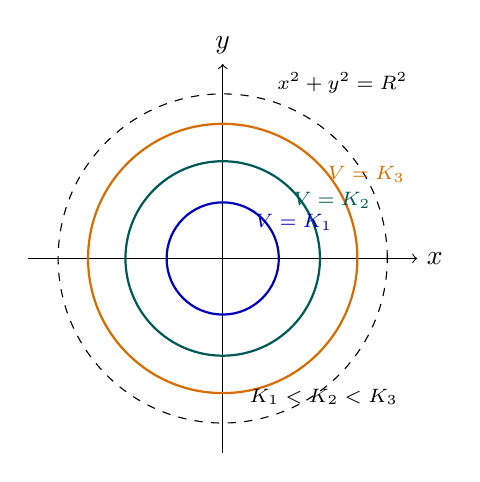
\begin{tikzpicture}[scale=0.95]
  \draw[->] (-2.6,0) -- (2.6,0) node[right] {\(x\)};
  \draw[->] (0,-2.6) -- (0,2.6) node[above] {\(y\)};

  \draw[dashed] (0,0) circle[radius=2.2];
  \node at (1.60,2.35) {\scriptsize \(x^2+y^2=R^2\)};

  \draw[thick,blue!75!black] (0,0) circle[radius=0.75];
  \draw[thick,teal!70!black] (0,0) circle[radius=1.30];
  \draw[thick,orange!85!black] (0,0) circle[radius=1.80];

  \node[blue!75!black] at (0.95,0.48) {\scriptsize \(V=K_1\)};
  \node[teal!70!black] at (1.46,0.78) {\scriptsize \(V=K_2\)};
  \node[orange!85!black] at (1.92,1.12) {\scriptsize \(V=K_3\)};
  \node at (1.35,-1.85) {\scriptsize \(K_1<K_2<K_3\)};
\end{tikzpicture}
\end{center}
\end{solutionbox}

\problem{prob:14-1-78}{78}{Investigate the family of surfaces
\[
z=(ax^2+by^2)e^{-x^2-y^2}.
\]
How does the shape of the graph depend on the numbers \(a\) and \(b\)?}

\begin{solutionbox}
\textbf{Method 1: Separate the radial part from the directional part}

\begin{steps}
\item Write the surface in polar-style variables
\[
x=\rho\cos\theta,\qquad y=\rho\sin\theta.
\]
Then
\[
z=\rho^2 e^{-\rho^2}\bigl(a\cos^2\theta+b\sin^2\theta\bigr).
\]
This is the right change of viewpoint because it separates ``how far from the origin'' from ``which direction''.

\item Define
\[
h(\rho)=\rho^2e^{-\rho^2}.
\]
Then
\[
h(0)=0,\qquad h(\rho)>0\ (\rho>0),\qquad h(\rho)\to 0\ \text{as}\ \rho\to\infty.
\]
Also
\[
h'(\rho)=2\rho e^{-\rho^2}(1-\rho^2),
\]
so \(h\) increases on \(0<\rho<1\), decreases on \(\rho>1\), and has its maximum at
\[
\rho=1,\qquad h(1)=\frac1e.
\]
Thus along every fixed ray from the origin, the graph starts at \(0\), reaches its extreme height or depth at distance \(1\), and then decays back toward \(0\).

\item The only part depending on direction is
\[
m(\theta)=a\cos^2\theta+b\sin^2\theta.
\]
This quantity always lies between \(\min(a,b)\) and \(\max(a,b)\). Therefore the signs and relative sizes of \(a\) and \(b\) control the whole shape.

\item If \(a,b>0\), then \(m(\theta)>0\) for every direction, so the whole surface lies above the \(xy\)-plane except at the origin and at infinity where it tends to \(0\). It is a positive mound. The largest crest occurs in the direction of the larger coefficient:
\[
\max z=\frac{\max(a,b)}{e}.
\]
If \(a=b>0\), the graph is rotationally symmetric and the crest is the whole circle \(\rho=1\).

\item If \(a,b<0\), then the graph is the upside-down version: it lies below the plane and forms a trough. The deepest point value is
\[
\min z=\frac{\min(a,b)}{e}.
\]
If \(a=b<0\), the trough is again circular.

\item If \(ab<0\), then \(m(\theta)\) changes sign. So the surface has positive humps in some directions and negative dips in others. The zero set is determined by
\[
ax^2+by^2=0,
\]
which gives two lines through the origin. In this case the origin is a saddle point.

\item If one coefficient is zero, say \(b=0\), then
\[
z=ax^2e^{-x^2-y^2}.
\]
The whole \(y\)-axis becomes part of the zero set, and the surface forms two humps or two dips along the \(x\)-direction, depending on the sign of \(a\). The case \(a=0\) is analogous with the roles of \(x\) and \(y\) reversed.
\end{steps}
\end{solutionbox}

\begin{solutionbox}
\textbf{Method 2: Locate the critical points}

\begin{steps}
\item Let
\[
q=ax^2+by^2,\qquad s=x^2+y^2.
\]
Then
\[
z=qe^{-s}.
\]
Differentiate:
\[
z_x=2xe^{-s}(a-q),\qquad z_y=2ye^{-s}(b-q).
\]
This method is appropriate because critical points tell us where peaks, dips, and saddles can occur.

\item The equations \(z_x=0\) and \(z_y=0\) give the critical points. We always have
\[
(0,0).
\]
Also, if \(a\ne 0\), then \(y=0\) and \(q=a\) give
\[
(\pm 1,0),
\qquad z=\frac{a}{e}.
\]
If \(b\ne 0\), then \(x=0\) and \(q=b\) give
\[
(0,\pm 1),
\qquad z=\frac{b}{e}.
\]

\item If \(a=b\), then the conditions \(q=a\) and \(q=b\) are the same, so every point on
\[
x^2+y^2=1
\]
is critical. That exactly matches the circular ridge or circular trench found in Method 1.

\item Near the origin,
\[
e^{-x^2-y^2}=1+o(1),
\]
so
\[
z\sim ax^2+by^2.
\]
Therefore the origin is:
\begin{itemize}
\item a local minimum if \(a,b>0\),
\item a local maximum if \(a,b<0\),
\item a saddle if \(ab<0\),
\item flat in one axis direction if one coefficient is \(0\).
\end{itemize}

\item The values at \((\pm1,0)\) and \((0,\pm1)\) show where the largest humps or deepest dips occur when \(a\ne b\). The larger coefficient gives the higher pair of peaks, and the smaller coefficient gives the lower pair of valleys. This confirms the full classification from Method 1.
\end{steps}
\end{solutionbox}

\begin{solutionbox}
\textbf{Hand-in Version}

Write
\[
x=\rho\cos\theta,\qquad y=\rho\sin\theta.
\]
Then
\[
z=\rho^2e^{-\rho^2}\bigl(a\cos^2\theta+b\sin^2\theta\bigr).
\]
The radial factor \(\rho^2e^{-\rho^2}\) is always \(\ge 0\), equals \(0\) at \(\rho=0\), tends to \(0\) as \(\rho\to\infty\), and is largest when \(\rho=1\). So along every direction, the surface rises or falls from \(0\), reaches its extreme value at distance \(1\), and then decays back toward \(0\).

Therefore the shape is controlled by
\[
a\cos^2\theta+b\sin^2\theta.
\]
So:
\begin{itemize}
\item If \(a,b>0\), the graph is entirely above the \(xy\)-plane, with peaks on the unit circle. If \(a=b\), it is rotationally symmetric with a circular ridge.
\item If \(a,b<0\), the graph is entirely below the plane; if \(a=b\), it has a circular trench.
\item If \(ab<0\), the graph has both positive and negative parts, the origin is a saddle, and the zero set includes the two lines \(ax^2+by^2=0\).
\item If one of \(a,b\) is \(0\), then one coordinate axis belongs to the zero set, and the graph has humps or dips only in the other direction.
\end{itemize}

The key critical values are
\[
z(\pm1,0)=\frac{a}{e},\qquad z(0,\pm1)=\frac{b}{e},
\]
so the larger coefficient determines the higher peaks and the smaller coefficient determines the lower valleys.
\end{solutionbox}

\sectiontitle{sec:14-2}{14-2}

\problem{prob:14-2-23}{23}{Find the limit, if it exists, or show that the limit does not exist.
\[
\lim_{(x,y)\to(0,0)} \frac{xy^2\cos y}{x^2+y^4}
\]}

\begin{solutionbox}
\textbf{Method 1: Compare two carefully chosen paths}

\begin{steps}
\item The denominator contains \(x^2+y^4\), so a natural comparison is to choose paths where \(x\) has the same size as \(y^2\). That is why the parabola \(x=cy^2\) is a useful family here.

\item First choose
\[
x=y^2.
\]
Then
\[
\frac{xy^2\cos y}{x^2+y^4}
\;=\;
\frac{y^2\cdot y^2\cos y}{y^4+y^4}
\;=\;
\frac{\cos y}{2}
\;\longrightarrow\;
\frac12.
\]

\item Next choose
\[
x=-y^2.
\]
Then
\[
\frac{xy^2\cos y}{x^2+y^4}
\;=\;
\frac{-y^2\cdot y^2\cos y}{y^4+y^4}
\;=\;
-\frac{\cos y}{2}
\;\longrightarrow\;
-\frac12.
\]

\item Since two paths approaching \((0,0)\) give two different limiting values, the limit does not exist. This is decisive because a multivariable limit, if it exists, must be the same along every path.
\end{steps}
\end{solutionbox}

\begin{solutionbox}
\textbf{Method 2: Use the whole path family \(x=ky^2\)}

\begin{steps}
\item Let
\[
x=ky^2,
\]
where \(k\) is any constant. This is a stronger version of Method 1 because it tests infinitely many paths at once.

\item Substituting gives
\[
\frac{xy^2\cos y}{x^2+y^4}
\;=\;
\frac{(ky^2)y^2\cos y}{k^2y^4+y^4}
\;=\;
\frac{k\cos y}{k^2+1}.
\]

\item As \(y\to 0\), we obtain
\[
\lim_{y\to 0}\frac{k\cos y}{k^2+1}
\;=\;
\frac{k}{k^2+1}.
\]
This limiting value depends on \(k\).

\item For example, \(k=1\) gives \(\frac12\), while \(k=-1\) gives \(-\frac12\). Because the value depends on the chosen path parameter \(k\), the two-variable limit cannot exist.
\end{steps}
\end{solutionbox}

\begin{solutionbox}
\textbf{Hand-in Version}

Take the paths \(x=y^2\) and \(x=-y^2\).

If \(x=y^2\), then
\[
\frac{xy^2\cos y}{x^2+y^4}
=\frac{y^2\cdot y^2\cos y}{y^4+y^4}
=\frac{\cos y}{2}\to \frac12.
\]

If \(x=-y^2\), then
\[
\frac{xy^2\cos y}{x^2+y^4}
=\frac{-y^2\cdot y^2\cos y}{y^4+y^4}
=-\frac{\cos y}{2}\to -\frac12.
\]

Since these two paths give different values, the limit does not exist:
\[
\boxed{\text{the limit does not exist}.}
\]
\end{solutionbox}

\problem{prob:14-2-24}{24}{Find the limit, if it exists, or show that the limit does not exist.
\[
\lim_{(x,y)\to(0,0)} \frac{x^3-y^3}{x^2+xy+y^2}
\]}

\begin{solutionbox}
\textbf{Method 1: Factor the numerator}

\begin{steps}
\item Use the algebraic identity
\[
x^3-y^3=(x-y)(x^2+xy+y^2).
\]
This is the most natural first move because the denominator already contains the same quadratic factor.

\item For \((x,y)\ne(0,0)\), the denominator
\[
x^2+xy+y^2
\]
is never \(0\). Indeed,
\[
2(x^2+xy+y^2)=(x+y)^2+x^2+y^2>0
\]
unless \(x=y=0\).

\item Therefore, for all \((x,y)\ne(0,0)\),
\[
\frac{x^3-y^3}{x^2+xy+y^2}=x-y.
\]
This is the key simplification: the complicated quotient is actually just a linear expression near the origin.

\item Now take the limit:
\[
\lim_{(x,y)\to(0,0)}(x-y)=0.
\]
So the original limit exists and equals \(0\).
\end{steps}
\end{solutionbox}

\begin{solutionbox}
\textbf{Method 2: Estimate the quotient directly}

\begin{steps}
\item Start with
\[
\left|\frac{x^3-y^3}{x^2+xy+y^2}\right|
\le
\frac{|x|^3+|y|^3}{x^2+xy+y^2}.
\]
This method is appropriate because if we can squeeze the absolute value to \(0\), then the limit must be \(0\).

\item The denominator has the lower bound
\[
2(x^2+xy+y^2)=(x+y)^2+x^2+y^2\ge x^2+y^2,
\]
so
\[
x^2+xy+y^2\ge \frac12(x^2+y^2).
\]

\item Also,
\[
|x|^3\le (x^2+y^2)^{3/2},
\qquad
|y|^3\le (x^2+y^2)^{3/2},
\]
so
\[
|x|^3+|y|^3\le 2(x^2+y^2)^{3/2}.
\]

\item Combining these inequalities,
\[
\left|\frac{x^3-y^3}{x^2+xy+y^2}\right|
\le
\frac{2(x^2+y^2)^{3/2}}{\frac12(x^2+y^2)}
=4\sqrt{x^2+y^2}\to 0.
\]
Hence the limit is \(0\).
\end{steps}
\end{solutionbox}

\begin{solutionbox}
\textbf{Hand-in Version}

Factor the numerator:
\[
x^3-y^3=(x-y)(x^2+xy+y^2).
\]
Since
\[
x^2+xy+y^2=0
\]
only at \((0,0)\), we may cancel for all nearby points \((x,y)\ne(0,0)\):
\[
\frac{x^3-y^3}{x^2+xy+y^2}=x-y.
\]
Therefore
\[
\lim_{(x,y)\to(0,0)} \frac{x^3-y^3}{x^2+xy+y^2}
=
\lim_{(x,y)\to(0,0)}(x-y)=0.
\]
So
\[
\boxed{0}
\]
is the limit.
\end{solutionbox}

\problem{prob:14-2-30}{30}{Find the limit, if it exists, or show that the limit does not exist.
\[
\lim_{(x,y,z)\to(0,0,0)} \frac{x^4+y^2+z^3}{x^4+2y^2+z}
\]}

\begin{solutionbox}
\textbf{Method 1: Compare two simple paths}

\begin{steps}
\item The denominator contains terms \(x^4\), \(y^2\), and \(z\), so a good first test is to isolate one variable at a time. This often reveals whether the limit can even be unique.

\item Along the \(x\)-axis, take
\[
y=0,\qquad z=0.
\]
Then
\[
\frac{x^4+y^2+z^3}{x^4+2y^2+z}
=\frac{x^4}{x^4}=1
\]
for \(x\ne 0\). So along this path the limit is \(1\).

\item Along the \(z\)-axis, take
\[
x=0,\qquad y=0.
\]
Then
\[
\frac{x^4+y^2+z^3}{x^4+2y^2+z}
=\frac{z^3}{z}=z^2\to 0.
\]

\item Since the path limits are different, the three-variable limit does not exist.
\end{steps}
\end{solutionbox}

\begin{solutionbox}
\textbf{Method 2: Use a one-parameter family of paths}

\begin{steps}
\item Let
\[
y=0,\qquad z=\lambda x^4,
\]
where \(\lambda\) is a constant with \(\lambda\ne -1\). This family is useful because it keeps the two dominant denominator terms \(x^4\) and \(z\) of the same order.

\item Substituting gives
\[
\frac{x^4+y^2+z^3}{x^4+2y^2+z}
=
\frac{x^4+\lambda^3x^{12}}{x^4+\lambda x^4}
=
\frac{1+\lambda^3x^8}{1+\lambda}.
\]

\item As \(x\to 0\),
\[
\frac{1+\lambda^3x^8}{1+\lambda}\to \frac{1}{1+\lambda}.
\]
So the limiting value depends on \(\lambda\).

\item For example,
\[
\lambda=0 \Rightarrow 1,
\qquad
\lambda=1 \Rightarrow \frac12.
\]
Because different paths give different answers, the limit cannot exist.
\end{steps}
\end{solutionbox}

\begin{solutionbox}
\textbf{Hand-in Version}

Along the path \(y=0,\ z=0\),
\[
\frac{x^4+y^2+z^3}{x^4+2y^2+z}
=\frac{x^4}{x^4}=1.
\]

Along the path \(x=0,\ y=0\),
\[
\frac{x^4+y^2+z^3}{x^4+2y^2+z}
=\frac{z^3}{z}=z^2\to 0.
\]

Since the two path limits are different, the limit does not exist:
\[
\boxed{\text{the limit does not exist}.}
\]
\end{solutionbox}

\problem{prob:14-2-42}{42}{Determine the set of points at which the function is continuous.
\[
F(x,y)=\cos\sqrt{1+x-y}
\]}

\begin{solutionbox}
\textbf{Method 1: Use continuity of a composition}

\begin{steps}
\item The outer function \(\cos u\) is continuous for every real \(u\). The inner function \(\sqrt{v}\) is continuous for \(v\ge 0\). So the only issue is where
\[
1+x-y
\]
is nonnegative.

\item Therefore the natural domain is
\[
1+x-y\ge 0
\qquad\Longleftrightarrow\qquad
y\le x+1.
\]
This step is appropriate because a composition of continuous functions is continuous exactly where every stage is defined.

\item On that half-plane, the function
\[
(x,y)\mapsto 1+x-y
\]
is continuous, then
\[
(x,y)\mapsto \sqrt{1+x-y}
\]
is continuous because its input stays in \([0,\infty)\), and then applying cosine preserves continuity.

\item The boundary line
\[
y=x+1
\]
is included, because then the square-root input is \(0\), and \(\sqrt{0}\) and \(\cos 0\) are both perfectly well defined.
\end{steps}
\end{solutionbox}

\begin{solutionbox}
\textbf{Method 2: Check interior, boundary, and exterior separately}

\begin{steps}
\item If
\[
1+x_0-y_0>0,
\]
then the point lies strictly inside the region where the square root is defined. By continuity of \(1+x-y\), nearby points still satisfy \(1+x-y>0\), so \(F\) is continuous there.

\item If
\[
1+x_0-y_0=0,
\]
then the point lies on the boundary line \(y=x+1\). Near that point, the expression \(1+x-y\) stays nonnegative on the domain side, and \(\sqrt{t}\) is continuous at \(t=0\). Therefore \(F\) is also continuous at boundary points.

\item If
\[
1+x_0-y_0<0,
\]
then \(\sqrt{1+x_0-y_0}\) is not real, so the function is not defined there and cannot be continuous there.

\item Combining the three cases gives the full continuity set.
\end{steps}
\end{solutionbox}

\begin{solutionbox}
\textbf{Hand-in Version}

The function
\[
F(x,y)=\cos\sqrt{1+x-y}
\]
is defined exactly when
\[
1+x-y\ge 0,
\]
that is,
\[
y\le x+1.
\]
On this set, the functions
\[
1+x-y,\qquad \sqrt{\phantom{u}},\qquad \cos
\]
are composed in a valid way, and each step is continuous. The boundary line \(y=x+1\) is included because \(\sqrt{0}\) is defined.

Hence \(F\) is continuous at exactly the points
\[
\boxed{\{(x,y): y\le x+1\}.}
\]
\end{solutionbox}

\problem{prob:14-2-48}{48}{Determine the set of points at which the function is continuous.
\[
f(x,y,z)=\sqrt{y-x^2}\ln z
\]}

\begin{solutionbox}
\textbf{Method 1: Find the domain, then use continuity rules}

\begin{steps}
\item The factor
\[
\sqrt{y-x^2}
\]
is defined when
\[
y-x^2\ge 0.
\]
The factor
\[
\ln z
\]
is defined when
\[
z>0.
\]
So the domain is
\[
y\ge x^2,\qquad z>0.
\]

\item This is the correct place to start because the product of continuous functions is continuous wherever both factors are defined and continuous.

\item On the set
\[
\{(x,y,z): y\ge x^2,\ z>0\},
\]
the square-root factor is continuous and the logarithm factor is continuous, so their product is continuous.

\item The boundary \(y=x^2\) is included, since \(\sqrt{0}=0\). But the plane \(z=0\) is not included, because \(\ln z\) is not defined there.
\end{steps}
\end{solutionbox}

\begin{solutionbox}
\textbf{Method 2: Analyze each defining restriction geometrically}

\begin{steps}
\item The condition
\[
y\ge x^2
\]
means the point must lie on or above the parabolic cylinder \(y=x^2\). This is the region where the square root is real.

\item The condition
\[
z>0
\]
means the point must lie in the open half-space above the plane \(z=0\). This is the region where the logarithm exists.

\item A point is in the continuity set exactly when it satisfies both restrictions at once, because then every nearby point in the domain keeps the same valid inputs for the square root and logarithm.

\item Therefore the continuity set is the intersection of those two regions: on or above the parabolic cylinder, and strictly above the plane \(z=0\).
\end{steps}
\end{solutionbox}

\begin{solutionbox}
\textbf{Hand-in Version}

For
\[
f(x,y,z)=\sqrt{y-x^2}\ln z,
\]
the square-root factor requires
\[
y-x^2\ge 0,
\]
and the logarithm requires
\[
z>0.
\]
On this domain, both factors are continuous, so their product is continuous there as well.

Therefore \(f\) is continuous exactly on
\[
\boxed{\{(x,y,z): y\ge x^2,\ z>0\}.}
\]
\end{solutionbox}

\problem{prob:14-2-49}{49}{Determine the set of points at which the function is continuous.
\[
f(x,y)=
\begin{cases}
\dfrac{x^2y^3}{2x^2+y^2}, & (x,y)\ne(0,0), \\
1, & (x,y)=(0,0).
\end{cases}
\]}

\begin{solutionbox}
\textbf{Method 1: Check the origin by squeezing the limit}

\begin{steps}
\item For \((x,y)\ne(0,0)\), the denominator
\[
2x^2+y^2>0,
\]
so the formula
\[
\frac{x^2y^3}{2x^2+y^2}
\]
is a quotient of continuous functions with nonzero denominator. Therefore the function is continuous everywhere except possibly at the origin.

\item To test the origin, estimate
\[
\left|\frac{x^2y^3}{2x^2+y^2}\right|.
\]
Since
\[
2x^2+y^2\ge y^2,
\]
we get
\[
\left|\frac{x^2y^3}{2x^2+y^2}\right|
\le
x^2|y|.
\]
This is the right estimate because the denominator removes two powers of \(y\), leaving a clearly small quantity.

\item Now
\[
x^2|y|
\le
(x^2+y^2)\sqrt{x^2+y^2}
=(x^2+y^2)^{3/2}\to 0
\]
as \((x,y)\to(0,0)\). Hence
\[
\lim_{(x,y)\to(0,0)} \frac{x^2y^3}{2x^2+y^2}=0.
\]

\item But the function value at the origin is defined to be
\[
f(0,0)=1.
\]
Since the limit is \(0\ne 1\), the function is not continuous at the origin.
\end{steps}
\end{solutionbox}

\begin{solutionbox}
\textbf{Method 2: Use polar coordinates at the origin}

\begin{steps}
\item Again, away from \((0,0)\) the rational formula is continuous, so only the origin needs attention.

\item Put
\[
x=r\cos\theta,\qquad y=r\sin\theta.
\]
Then for \(r>0\),
\[
\frac{x^2y^3}{2x^2+y^2}
=
\frac{r^2\cos^2\theta\cdot r^3\sin^3\theta}{2r^2\cos^2\theta+r^2\sin^2\theta}
=
r^3\frac{\cos^2\theta\sin^3\theta}{2\cos^2\theta+\sin^2\theta}.
\]

\item The angular factor is bounded, because
\[
2\cos^2\theta+\sin^2\theta=1+\cos^2\theta\ge 1.
\]
So
\[
\left|r^3\frac{\cos^2\theta\sin^3\theta}{2\cos^2\theta+\sin^2\theta}\right|
\le r^3.
\]

\item Therefore the limit of the rational part at the origin is \(0\). Since the piecewise definition assigns the value \(1\) at \((0,0)\), the function fails to be continuous there.
\end{steps}
\end{solutionbox}

\begin{solutionbox}
\textbf{Hand-in Version}

For \((x,y)\ne(0,0)\),
\[
f(x,y)=\frac{x^2y^3}{2x^2+y^2}
\]
is continuous because \(2x^2+y^2>0\).

At the origin,
\[
\left|\frac{x^2y^3}{2x^2+y^2}\right|
\le x^2|y|
\le (x^2+y^2)^{3/2}\to 0.
\]
So
\[
\lim_{(x,y)\to(0,0)} \frac{x^2y^3}{2x^2+y^2}=0.
\]
But
\[
f(0,0)=1.
\]
Therefore \(f\) is not continuous at \((0,0)\), and it is continuous everywhere else.

Hence the continuity set is
\[
\boxed{\mathbb{R}^2\setminus\{(0,0)\}.}
\]
\end{solutionbox}

\end{document}
